\subsection{Pretraining Data}
\label{sec:pretrain_data}

\subsubsection{Data}

We describe here several new datasets that we added to pretraining since Nemotron 3 Nano~\citep{nvidia2025nemotron3nanoopen}. We are releasing these datasets on HuggingFace as  \href{https://huggingface.co/datasets/nvidia/Nemotron-Pretraining-Specialized-v1.1}{\texttt{Nemotron-Pretraining-Specialized-v1.1}}.

\subsubsection{Synthetic Code Concepts}
With the aim of improving Python problem-solving capabilities, we synthetically generated a dataset consisting Python problems and solutions. Using a taxonomy consisting of thousands of programming concepts curated from our \href{https://huggingface.co/datasets/nvidia/Nemotron-Pretraining-code-v1}{\texttt{Nemotron-Pretraining-Code}} datasets and GPT-OSS-120B, we extracted high-level programming concepts from the HumanEval benchmark dataset \citep{chen2021evaluatinglargelanguagemodels}. In total, after deduplication of the extracted taxonomical representations, we collected a total of 91 concepts.

Using the extracted concepts, we performed open-ended generation using GPT-OSS 20B to generate Python programming problems that test these concepts and instructed it to generate the problem with a descriptive function name and problem description in the function docstring. To generate these problems at the pretraining scale, we combined up to four concepts per generation and generated up to five problems per set of concepts. This resulted in a total of approximately 14 million problems.

Following problem generation, we then used GPT-OSS 120B to generate five self-contained solutions for each generated problem. To avoid biasing models trained on these data to generate long-winded solutions, we instructed GPT-OSS 120B to restrict its solution to 60 lines maximum. For each problem, we generate five solutions, and we stopped generating after obtaining approximately 23 million problem-solution pairs.

As a final step in generating this dataset, we thoroughly cleaned the generated problem-solution pairs. Our cleaning consisted of the following steps: we check that GPT-OSS-120 B did not include additional imports that were not specified in the original problem generated from GPT-OSS-20 B. We discard all solutions that did not satisfy this condition.
We form the final problem-solution pair by parsing only the solution provided by GPT-OSS-120B and appending it to the problem generated from GPT-OSS-20 B. We found that GPT-OSS-120B frequently modified the original problem and this ensured we maintained the desired format prescribed in our original problem-formation prompt.
We check that the final problem-solution pair is valid Python code via generation of an abstract-syntax tree (AST). If the final function does not pass the final AST check, it is discarded.
After the above cleaning procedure, we resulted in the 15 M problems that make up the dataset.

%Add ablation study


\subsubsection{Synthetic Unconditional Algorithmic}
% Markus, on behalf of Benedikt who left NVIDIA
To create this dataset, we generated algorithmic Python problems using Qwen3-235B-A22B (the base model) and gpt-oss-120b. We used minimalistic prompts---such as ``Write a function,'' ``Write a Python function,'' or ``Write a coding problem and solution for a student to solve''---and optionally specified a difficulty level (easy, medium, or hard). To ensure diversity and quality, we prompted gpt-oss-120b to rewrite these samples to handle edge cases, add unit tests, and reformat the outputs in various ways.

In another variant, we instructed gpt-oss-120b to generate LeetCode-style questions and answers, again with a randomly selected difficulty level. We further used gpt-oss-120b to score the correctness of the solution and, if incorrect, to correct it. Overall, such nearly unconditional prompting did result in high rates of duplicates. To combat this, we found it effective to deduplicate based on short titles of around 5--8 words generated by gpt-oss-120b for each problem.

All samples were decontaminated against HumanEval~\citep{chen2021evaluatinglargelanguagemodels}, MBPP~\citep{austin2021programsynthesislargelanguage}, CRUXEval~\citep{gu2024cruxevalbenchmarkcodereasoning}, and LiveCodeBench~\citep{jain2024livecodebench} as follows: First, exact matches of the solution against those benchmarks were removed. Second, we used Qwen3-Embedding-0.6 to encode Problem and Solution and filtered any data with >0.8 similarity with any of the benchmarks.

Although this dataset is small by usual pretraining standards (0.2B tokens), we believe it helps to teach coding practices like edge case handling and reasoning about program execution, as evidenced by improvements of 1-2 points to HumanEval, MBPP, and CRUXEval-O over the Nemotron 3 Nano base checkpoint, when adding these datasets to a redo of the last 100B tokens of 25T token pretraining.

\subsubsection{Synthetic Economics}
% \todo{Ying Lin - replace with a full description}

We generated a diverse set of economics multiple-choice questions across various formats, including cloze, calculation, sentence completion, and multiple-response, covering key topics and terms in microeconomics, macroeconomics, and econometrics (e.g., ``Statistical Inference and Hypothesis Testing - Type I error'' and ``Inflation and the Price Level - Inflation rate'') from a curated list. For each topic-term pair, we used Qwen3-235B-A22B-Thinking-2507 to generate multiple questions, each accompanied by a detailed, step-by-step, and well-formatted solution. To enhance the diversity, we further prompted the model to create new and original questions using the initial outputs as reference points. Each question-solution pair underwent model-based verification for clarity, ambiguity, solvability and accuracy.


\subsubsection{Synthetic Formal Logic}
% \todo{Ying Lin - replace with a full description}
% Multiple choice questions and answers about formal logic, with and without chain-of-thought. Contains examples designed for several patterns, e.g., natural language to formal logic, formal logic to natural language, solving problems using truth table, etc.

We synthesized a set of formal logic problems and solutions spanning several tasks, such as translating between natural language and predicate or propositional logic, deriving the antecedents of conditional propositions, and solving logic problems using indirect or complete truth tables.
We introduced variability into the generated scenarios, premises, and formulas by incorporating random personas,\footnote{\url{https://huggingface.co/collections/nvidia/nemotron-personas}} letters, and/or logic connective (i.e., $\land$, $\lor$, $\supset$, $\equiv$, $\sim$) into the prompt.
We generated and evaluated the problems and solutions using Qwen3-235B-A22B-Thinking-2507.

\subsubsection{Synthetic Multiple Choice}
% \todo{Dan Su - replace with a full description}
% Multiple choice questions and answers about a variety of topics found in the MMLU auxiliary train dataset.

We construct a multiple-choice question (MCQ) dataset by bootstrapping from the MMLU auxiliary training set~\citep{hendryckstest2021}, which aggregates auxiliary MCQ data from sources such as ARC~\citep{allenai:arc}, MC\_TEST~\citep{richardson-etal-2013-mctest}, OpenBookQA~\citep{OpenBookQA2018}, and RACE~\citep{lai-etal-2017-race}, etc. Starting from each seed question, we generate multiple similar questions that follow the same task format and difficulty profile, along with corresponding answer options by prompting Qwen3-235B-A22B ~\citep{yang2025qwen3technicalreport}. In the second stage, we prompt the DeepSeek-V3~\citep{deepseekai2025deepseekv3technicalreport} model to solve each generated question by selecting an answer and providing the supporting knowledge or contextual reasoning underlying its choice. To improve answer reliability, we sample multiple independent solution generations for each question using different random seeds. We then apply majority voting over the generated answers to identify the most consistent choice, retaining only those samples whose final answer agrees with the majority and discarding inconsistent or incorrect instances.

Using this pipeline, we generate approximately 3.5M MMLU-style MCQ samples (\textasciitilde1.6B tokens) augmented with explicit, relevant knowledge or reasoning traces. We evaluate the impact of this data via ablation experiments by continued training the Nemotron-Nano-V3~\citep{nvidia2025nemotron3nanoopen} 24.9T-token checkpoint with an additional 100B tokens, out of which 1B tokens are from the generated MMLU-aux-train-SDG data. The results show consistent gains on most of the benchmarks: MMLU improves from 77.22 to 77.51, "MATH Level 5" from 78.55 to 79.05, AIME-2024 improved from 53.3 to 56.7, and MBPP from from 74.8 to 75.2. Performance on other benchmarks remains largely stable with only minor variance, indicating that the synthesized MCQ data primarily strengthens mathematical and structured reasoning capabilities without introducing regressions elsewhere.

\subsubsection{Data Mixture and Ordering}

We adopt the Nemotron 3 Nano data mixture as described in~\citep{nvidia2025nemotron3nanoopen}. Our pretraining corpus spans 16 high-level categories. The largest component is web crawl data, which we partition into five quality-based groups following the Nemotron-CC taxonomy~\citep{su2024nemotroncctransformingcommoncrawl}: crawl-medium, crawl-medium-high, and crawl-high, representing progressively higher-quality crawl data, along with their synthetic counterparts, syn-crawl-medium-high and syn-crawl-high, generated from filtered web documents.
Beyond web crawl, the mixture includes math~\citep{karimi2025nemotronccmath,akter2024mindmathinformedsynthetic}, Wikipedia, code, Nemotron-CC-Code, academic text, Crawl++, multilingual data, finepdfs~\citep{kydlicek2025finepdfs} and synthetic SFT-style datasets. The SFT-style data is further divided into general-sft, stem-sft, and code-sft. As part of the SFT-style component, we incorporate reasoning-focused datasets into pretraining, motivated by prior findings demonstrating their effectiveness~\citep{akter2026frontloading}. Crawl++ consists of OpenWebText, BigScience~\citep{laurencon2023bigsciencerootscorpus16tb}, and Reddit datasets.

Data blending is designed to balance diversity and quality: sources with comparable estimated quality are assigned similar weights, while higher-quality datasets receive proportionally greater weight in the mixture.
Further details on dataset quality estimation and mixture construction are provided in~\citep{feng2024maximizedataspotentialenhancing}.
We adopt the two-phase curriculum proposed in ~\citep{feng2024maximizedataspotentialenhancing} work. 
In Phase 1, the mixture emphasizes data diversity to promote broad coverage and generalization. 
In Phase 2, the blend shifts toward predominantly high-quality sources (e.g., Wikipedia) to refine model performance. 
The transition to Phase 2 occurs at 80\% of total training tokens. 
The specific mixtures used in each phase are illustrated in Figure~\ref{fig:pretrain-blends}.


\begin{figure}[htbp]
    \centering
    \begin{subfigure}{0.49\textwidth}
        \centering
        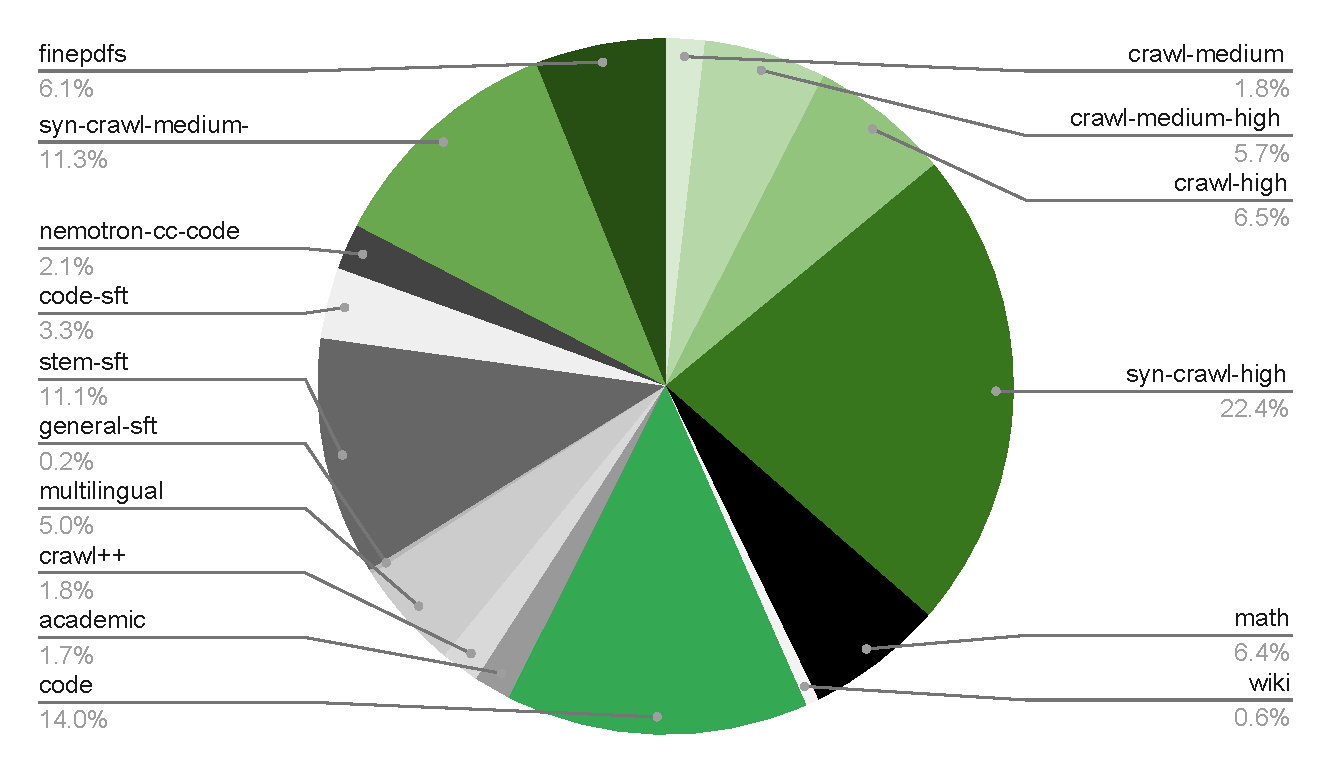
\includegraphics[width=\linewidth]{figures/super-phase1.pdf}
        \caption{Data mixture of Phase 1.}
        \label{fig:phase1-blend}
    \end{subfigure}
    \begin{subfigure}{0.49\textwidth}
        \centering
        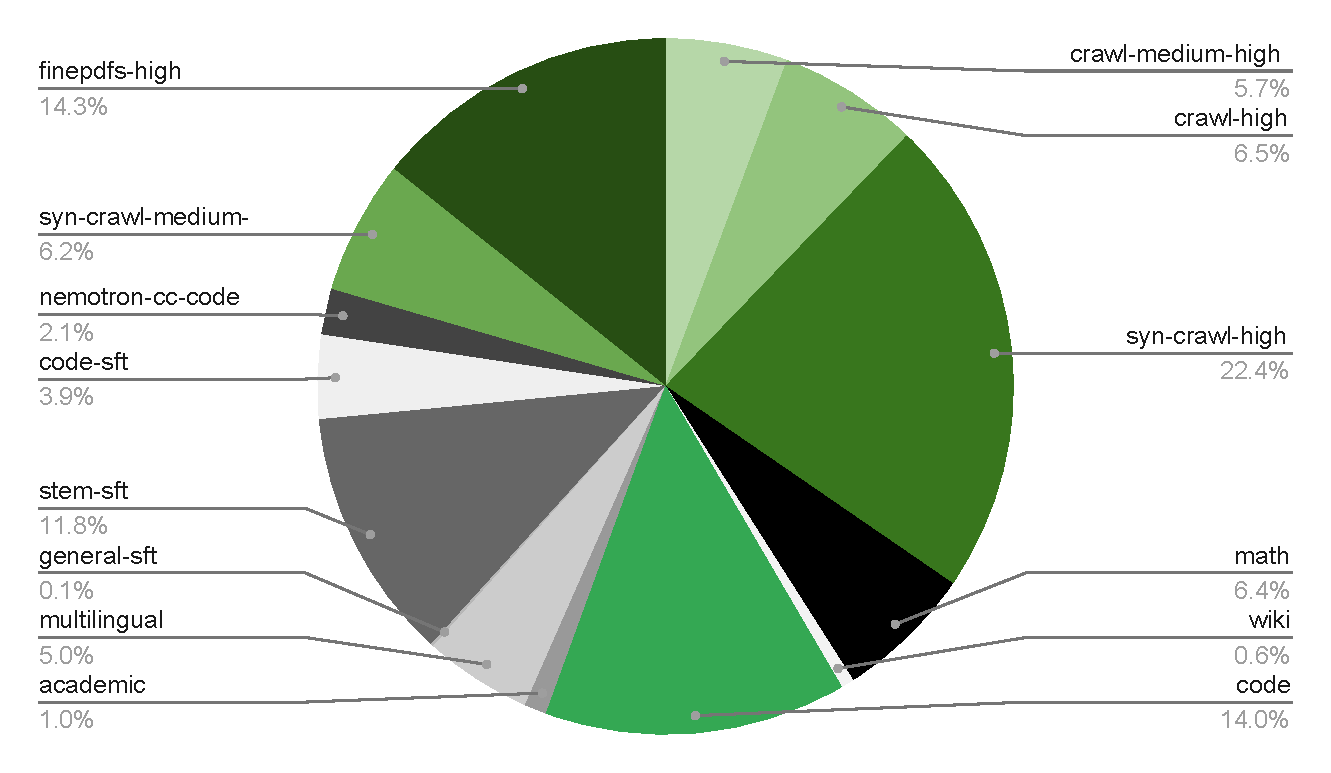
\includegraphics[width=\linewidth]{figures/super-phase2.pdf}
        \caption{Data mixture of Phase 2.}
        \label{fig:phase2-blend}
    \end{subfigure}
    \caption{Data mixtures for each phase of pre-training.}
    \label{fig:pretrain-blends}
\end{figure}

